\documentclass[10pt]{beamer}

\usepackage{graphicx}

\usetheme{metropolis}
\usepackage{appendixnumberbeamer}

\usepackage{booktabs}
\usepackage[scale=2]{ccicons}

\usepackage{pgfplots}
\usepgfplotslibrary{dateplot}

\usepackage{xspace}
\newcommand{\themename}{\textbf{\textsc{metropolis}}\xspace}

\usepackage{listings}
\usepackage{hyperref}

\title{Programming for Regional and City Planning}
\subtitle{Kuliah Umum - Architecture and Planning Department UGM}
\date{\today}
\author{\textbf{Dr. Bambang Purnomosidi D. P.}}
\institute{Master in Information Technology Department - STMIK Akakom\\PT Wabi Teknologi Indonesia}
%\titlegraphic{\hfill
\includegraphics[height=1.5cm]{isriti-logo.png}}

\begin{document}

\maketitle

\begin{frame}[allowframebreaks]{Table of contents}
  \setbeamertemplate{section in toc}[sections numbered]
  \setbeamertemplate{subsection in toc}{\leavevmode\leftskip=3.2em\rlap{\hskip-2em\inserttocsectionnumber.\inserttocsubsectionnumber}\inserttocsubsection\par}
  \tableofcontents
  %\tableofcontents[hideallsubsections]
\end{frame}

\section{About}

  \subsection{About Me}

    \begin{frame}[fragile]{Let's Get to Know Each Other}

      \begin{itemize}
        \item Ph.D from DTETI - UGM
        \item Lecturer at STMIK Akakom, head of Magister Teknologi Informasi 
        \item Programming since 18 years old - it’s been 30 years! 
        \item More in industry than in university, my latest tech position is Senior Software Architect.
        \item CEO at PT Wabi Teknologi Indonesia, a software engineering company
        \item Community involvement:
          \begin{itemize}
            \item Founded Rust Indonesia - and still maintains it.
            \item Founded Arch Linux Indonesia - and still maintians it
            \item KPLI, Ruby Indonesia: no longer active.
          \end{itemize}
        \item Certified in Blockchain from Corda, LSP digital assessor.
        \item I’m happiest when I’m coding
      \end{itemize}

    \end{frame}

  \subsection{About You}

    \begin{frame}[fragile]{It's A Sharing Session}

      I may know something you don't know, you may know something I don't know.

    \end{frame}

\section{The Big Picture}

  \subsection{Software Taxonomy}

    \begin{frame}[fragile]{Software Taxonomy}

      \begin{itemize}
        \item Operating System
        \item Development Tools
        \item Application Program
        \item Utilities
      \end{itemize}

    \end{frame}

  \subsection{Engineering a Software}

    \begin{frame}[fragile]{Engineering a Software}

      It's the domain of Software Engineering body of knowledge. Programming is substantial part but
      not the most important part. In fact, every part is important, lack of them will result in
      software defects.

%      \begin{figure}[h]
%      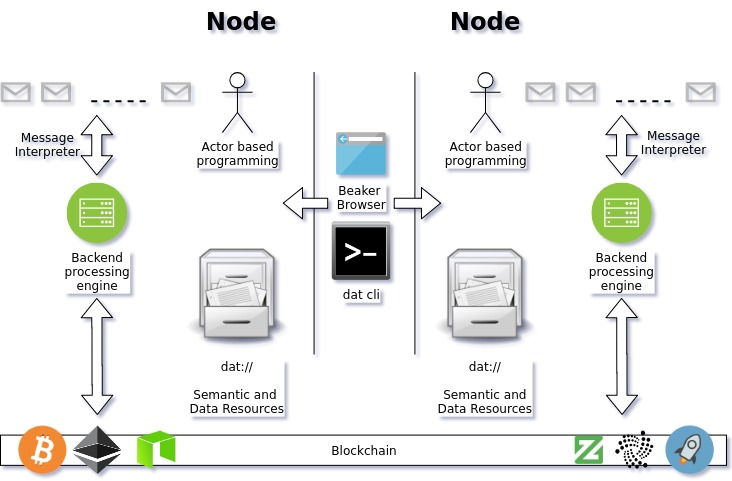
\includegraphics[scale=0.4]{decweb-pragmatic-int}
%      \end{figure}

    \end{frame}

\section{Programming: Coding, Algorithm, and Data Structure}

  \subsection{What is Programming?}

    \begin{frame}[fragile]{What is Programming?}

      \textbf{Programming}: using a language to instruct the computer to do {various tasks|a specific task}.

      Normally, machine can only read binary (1-0), so human need to understand 1-0. From the
      closeness of instruction to machine, we have:
      \begin{itemize}
        \item High-level language: understood by human, translated to machine understandble format
          (Python, Ruby, Java).
        \item Middle-level language: understood by human, hava a capability to embed machine code
          (C, Rust).
        \item Low-level language: very close to machine, using mnemonic (Assembly).
      \end{itemize}
    \end{frame}

  \subsection{How do I Program?}

    \begin{frame}[fragile]{How do I Program?}

      You need programming language(s) and development tools

    \end{frame}

  \subsection{Programming Languages and Development Tools}

    \begin{frame}[fragile]{Programming Languages and Development Tools}

      \begin{itemize}
        \item \textbf{Programming Languages (PL)}: formal language that specifies a set of instructions for computer to do something.
        \item PL should be seen from 2 points: specification and implementation (reference
          implementation and vendor implementation).
        \item \textbf{Development Tools (DT)}: a set of tools to help software developer in doing their tasks to create software product:
          \begin{itemize}
            \item IDE (Integrated Development Environment)
            \item Compiler / Interpreter
            \item Profiler
            \item Debugger
            \item Editor
            \item Package Management
            \item Programming Environemnt (discussed later)
          \end{itemize}
      \end{itemize}

    \end{frame}

  \subsection{Algorithm}

    \begin{frame}[fragile]{What is Algorithm?}

An algorithm is a finite sequence of well-defined, computer-implementable instructions, typically to
solve a class of problems or to perform a computation.

\textbf{Example}

Problem: Given a list of positive numbers, return the largest number on the list.

\begin{lstlisting}
Set max to 0.
For each number x in the list L, compare it to max. 
If x is larger, set max to x.
max is now set to the largest number in the list.
\end{lstlisting}

Python implementation:

\begin{lstlisting}[language=python]
    max = 0
    for x in L:
        if x > max:
            max = x
\end{lstlisting}

    \end{frame}

  \subsection{Data Structure}

    \begin{frame}[fragile]{Data Structure}

A data structure is a data organization, management, and storage format that enables efficient access and modification

\textbf{Niklaus Wirth}: Algorithms + Data Structures = Programs.

    \end{frame}

\section{Programming Paradigms}

  \subsection{What is Programming Paradigms?}

    \begin{frame}[fragile]{What is Programming Paradigms?}

      Programming Paradigm: related with the way programmers solve programming problem. PP are implemented as programming language features.

    \end{frame}

  \subsection{Some Programming Paradigms}

    \begin{frame}[fragile]{Some Programming Paradigms}

      \begin{itemize}
        \item \textbf{Imperative}: allow side effects, sequential, there are constructs to control order. Ex: Perl, Python, JavaScript, PHP
        \item \textbf{Functional Programming}: disallow side effects, treats computation as the evaluation of mathematical functions, avoids changing state and mutable data. Ex: Haskell, OCaml
        \item \textbf{Declarative}: order is not important, declare something and have computer do the work. Ex: SQL
        \item \textbf{Object Oriented Programming}: treat class as an encapsulation of executrable code and let the objects from the class to collaborate. Ex: Java, C++
        \item And many others
      \end{itemize}

      Current: multi paradigms.

    \end{frame}

\section{Programming Environment}

  \subsection{Programming Environment}

    \begin{frame}[fragile]{Programming Environment}

      \begin{itemize} 
        \item Programming is not the only thing to consider when we want to build software product.
        \item Programming environment are other things related to programming and DT, important for successful delivery of software products although may not be technically related. 
        \item It is the answer of: “I can program, I can do programming tasks, now how should I begin and how do I manage it so that I can deliver software product?”
      \end{itemize}

    \end{frame}

  \subsection{List of Programming Environment}

    \begin{frame}[fragile]{List of Programming Environment}
        Programming environment usually consists of:
          \begin{itemize}
            \item Software development methodology: waterfall, prototyping, agile.
            \item Cloud-enabled DT (platform as a service): Docker, Kubernetes, rkt, unikernel
            \item Distributed Computing: Data serialization: XML (OBSOLETE), JSON, msgpack, protocol buffer, etc.
            \item Testing and Continous Integration
            \item Online tools: workflow management (ex: trello), communication (Slack)
            \item Project Management: Github, Gitlab 
            \item Product Development: Aha (aha.io)
          \end{itemize}
    \end{frame}

  \subsection{Domain Problems}

    \begin{frame}[fragile]{Domain Problems}

        \begin{itemize}
          \item Frontend: GUI, TUI, and Web
          \item Mobile
          \item Backend - Distributed System: low latency Programming Language
          \item Programming Language - Compiler and libraries: microservices. 
          \item Data Technology: Big Data, SQL, NOSQL, NewSQL
          \item Big Data
          \item Artificial Intelligence: Machine Learning and Data Mining (ex: TensorFlow), Deep Learning: see Julia and R.
          \item Embedded System: Raspberry Pi etc: need specific OS and specific development tools: Python, Node.js, Rust, Go, C
        \end{itemize}
      \end{frame}

\section{Applying Programming for Regional and City Planning}

  \subsection{Some Notes on Software Engineering and Regional-City Planning}

    \begin{frame}[fragile]{Some Notes on Sofware Engineering and Regional-City Planning}

        \begin{itemize}
          \item I know almost nothing about regional - city planning, so, let's collaborate.
          \item Some papers - articles mention \textit{xxxxxxx algorithm} in regional-city planning
            related, but to have a fully functional solution, we should not neglect other IT things
            beside algorithm. 
        \end{itemize}

      \end{frame}

  \subsection{Some Ideas}

    \begin{frame}[fragile]{Some Ideas}
      \begin{itemize}
        \item Open Urban Planning Toolbox:
          \url{https://blogs.iadb.org/conocimiento-abierto/en/open-urban-planning-toolbox/}
        \item Regional Road Network Shortest Path Algorithm in Vehicle Navigation Systems: \url{https://link.springer.com/chapter/10.1007/978-3-642-53703-5\_36}
        \item Regional Road Network Shortest Path Algorithm in Vehicle Navigation Systems:
          \url{https://link.springer.com/chapter/10.1007/978-3-642-53703-5\_36}
        \item And many more.
      \end{itemize}
    \end{frame}

\end{document}

